


\documentclass{beamer}
\usetheme{ucl}

\usepackage[utf8]{inputenc}


%%% Increase the height of the banner: the argument is a scale factor >=1.0
%\setbeamertemplate{banner}[ucl][10.0]

%%% Change the colour of the main banner
%%% The background should be one of the UCL colours (except pink or white):
%%%   black,darkpurple,darkred,darkblue,darkgreen,darkbrown,richred,midred,
%%%   navyblue,midgreen,darkgrey,orange,brightblue,brightgreen,lightgrey,
%%%   lightpurple,yellow,lightblue,lightgreen,stone
\setbeamercolor{banner}{bg=darkpurple}
%\setbeamercolor{banner}{bg=yellow,fg=black}

%%% Add a stripe behind the banner
%\setbeamercolor{banner stripe}{bg=darkpurple,fg=black}

%%% The main structural elements
\setbeamercolor{structure}{fg=black}

%%% Author/Title/Date and slide number in the footline
\setbeamertemplate{footline}[author title date]

%%% Puts the section/subsection in the headline
% \setbeamertemplate{headline}[section]

%%% Puts a navigation bar on top of the banner
%%% For this to work correctly, the each \section command needs to be
%%% followed by a \subsection. Requires one extra compile.
% \setbeamertemplate{headline}[miniframes]
%%% Accepts an optional argument determining the width
% \setbeamertemplate{headline}[miniframes][0.3\paperwidth]


%%% Puts the frame title in the banner
%%% Won't work correctly with the above headline templates
%\useoutertheme{ucltitlebanner}
%%% Similar to above, but smaller (and puts subtitle on same line as title)
\useoutertheme[small]{ucltitlebanner}

%%% Gives block elements (theorems, examples) a border
% \useinnertheme{blockborder}
%%% Sets the body of block elements to be clear
% \setbeamercolor{block body}{bg=white,fg=black}

%%% Include CSML logo on title slide
%\titlegraphic{\includegraphics[width=0.16\paperwidth]{csml_logo}}

%%% Include CSML logo in bottom right corner of all slides
%\logo{\includegraphics[width=0.12\paperwidth]{csml_logo}}

%%% Set a background colour
% \setbeamercolor{background canvas}{bg=lightgrey}

%%% Set a background image
%%% Some sample images are available from the UCL image store:
%%%   https://www.imagestore.ucl.ac.uk/home/start
% \setbeamertemplate{background canvas}{%
%   \includegraphics[width=\paperwidth]{imagename}}



%%%%%% Some other settings that can make things look nicer
%%% Set a smaller indent for description environment
\setbeamersize{description width=2em}
%%% Remove nav symbols (and shift any logo down to corner)
\setbeamertemplate{navigation symbols}{\vspace{-2ex}}








\DeclareMathOperator{\Cov}{Cov}
\DeclareMathOperator{\Var}{Var}
\DeclareMathOperator{\E}{\mathbb{E}}
\DeclareMathOperator{\Proba}{\mathbb{P}}

\newcommand{\Covb}[2]{\ensuremath{\Cov\!\left[#1,#2\right]}}
\newcommand{\Eb}[1]{\ensuremath{\E\!\left[#1\right]}}
\newcommand{\Pb}[1]{\ensuremath{\Proba\!\left[#1\right]}}
\newcommand{\Varb}[1]{\ensuremath{\Var\!\left[#1\right]}}

% norm
\newcommand{\norm}[1]{\| #1 \|}

\newcommand{\indep}{\rotatebox[origin=c]{90}{$\models$}}





\usepackage{mathptmx,amsmath,amssymb,graphicx,bibentry,bbm,ragged2e}
\usepackage[english]{babel}

\makeatletter

\newcommand{\noun}[1]{\textsc{#1}}
\newcommand{\jitem}[1]{\item \begin{justify} #1 \end{justify} \vfill{}}
\newcommand{\sframe}[2]{\frame{\frametitle{#1} #2}}

\newenvironment{centercolumns}{\begin{columns}[c]}{\end{columns}}
%\newenvironment{jitem}{\begin{justify}\begin{itemize}}{\end{itemize}\end{justify}}



%\usetheme{Warsaw}
%\setbeamertemplate{footline}[text line]{}
%\setbeamertemplate{headline}{}
%\setbeamercolor{structure}{fg=purple!50!blue, bg=purple!50!blue}

%\setbeamersize{text margin left=15pt,text margin right=15pt}

%\setbeamercovered{transparent}


\@ifundefined{showcaptionsetup}{}{%
 \PassOptionsToPackage{caption=false}{subfig}}
\usepackage{subfig}

\usepackage[utf8]{inputenc}
\usepackage[T1]{fontenc}

\usepackage{multirow}


\makeatother

\def \draft {1}

\usepackage{xparse}
\usepackage{ifthen}
\DeclareDocumentCommand{\comment}{m o o o o}
{\ifthenelse{\draft=1}{
    \textcolor{red}{\textbf{C : }#1}
    \IfValueT{#2}{\textcolor{blue}{\textbf{A1 : }#2}}
    \IfValueT{#3}{\textcolor{ForestGreen}{\textbf{A2 : }#3}}
    \IfValueT{#4}{\textcolor{red!50!blue}{\textbf{A3 : }#4}}
    \IfValueT{#5}{\textcolor{Aquamarine}{\textbf{A4 : }#5}}
 }{}
}
\newcommand{\todo}[1]{
\ifthenelse{\draft=1}{\textcolor{red!50!blue}{\textbf{TODO : \textit{#1}}}}{}
}




\begin{document}


\title[MATSim Sensitivity analysis]{Sensitivity analysis of the MATSim transport model}

\author[Raimbault]{J.~Raimbault$^{1,2,3,\ast}$\\\medskip
$^{\ast}$\texttt{j.raimbault@ucl.ac.uk}
}

\institute[UCL]{$^{1}$Center for Advanced Spatial Analysis, University College London\\
$^{2}$UPS CNRS 3611 Complex Systems Institute Paris\\
$^{3}$UMR CNRS 8504 G{\'e}ographie-cit{\'e}s
}


\date[04/11/2021]{ECTQG 2021\\
Special Session: Exploration and validation of spatial simulation models\\
November 4th 2021
}

\frame{\maketitle}



\sframe{}{


\cite{cats2021multi}

\cite{szell2021growing}

\cite{cats2020modelling}



}



\sframe{Road network generation algorithm}{

At each time step, with a fixed population density: 

\begin{enumerate}
	\item Add new nodes preferentially to population and connect them
	\item \justify Variable heuristic for new links, among: nothing, random, gravity-based deterministic breakdown, gravity-based random breakdown (from \cite{schmitt2014modelisation}), cost-benefits (from \cite{louf2013emergence}), biological network generation (based on \cite{tero2010rules})
\end{enumerate}

\medskip

\centering

\frame{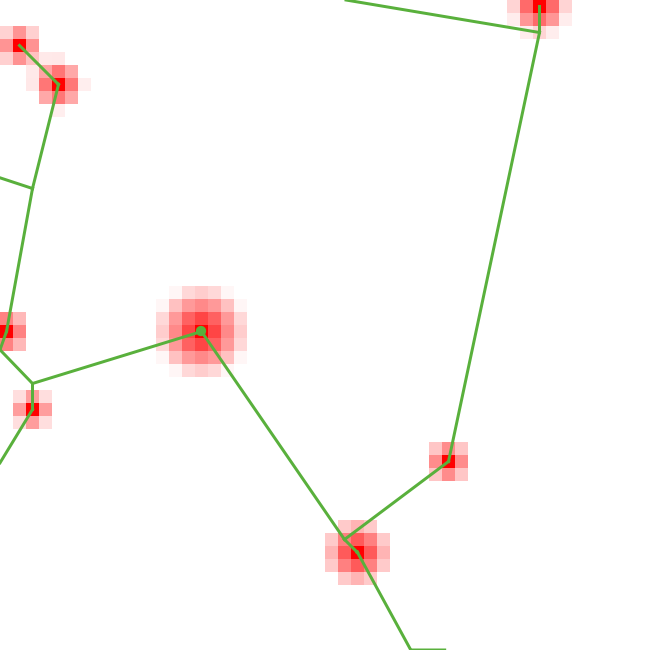
\includegraphics[width=0.32\textwidth]{figures/example_nwgrowth_tick0.png}}
\frame{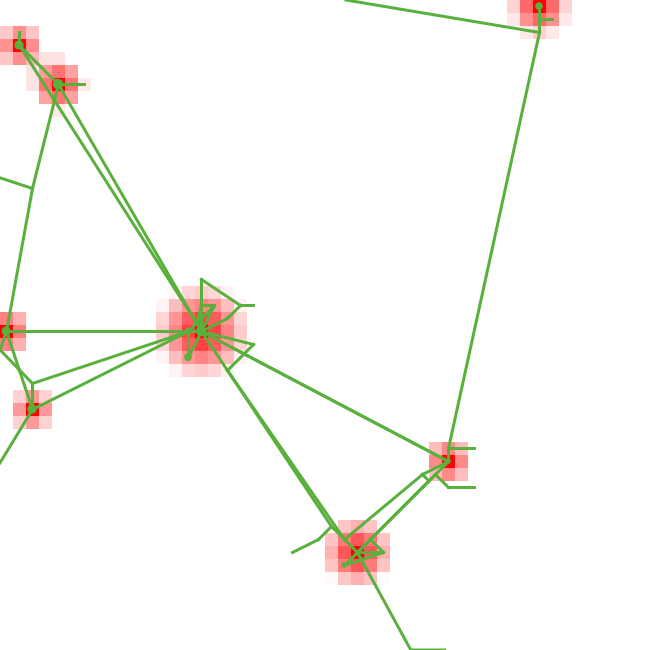
\includegraphics[width=0.32\textwidth]{figures/example_nwgrowth_tick2.png}}
\frame{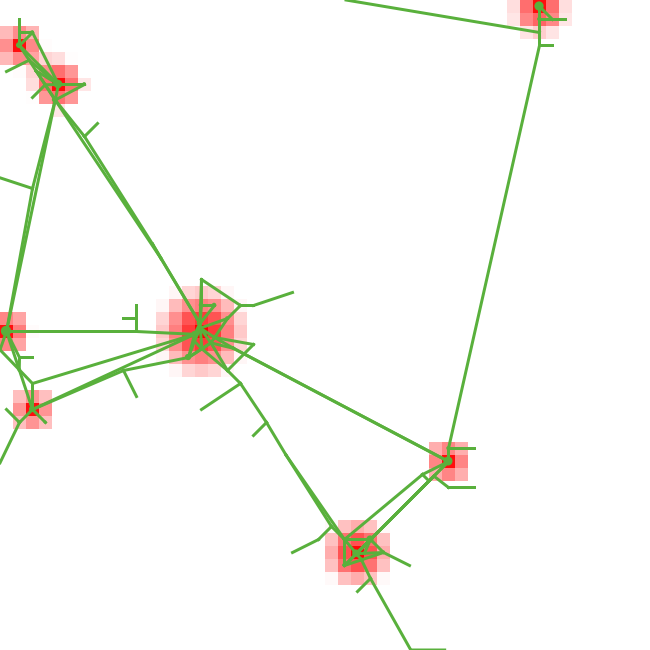
\includegraphics[width=0.32\textwidth]{figures/example_nwgrowth_tick10.png}}

}


\sframe{Biological network generation}{

Model studied by~\cite{tero2010rules} : exploration and reinforcement by a slime mould searching for ressources

\bigskip

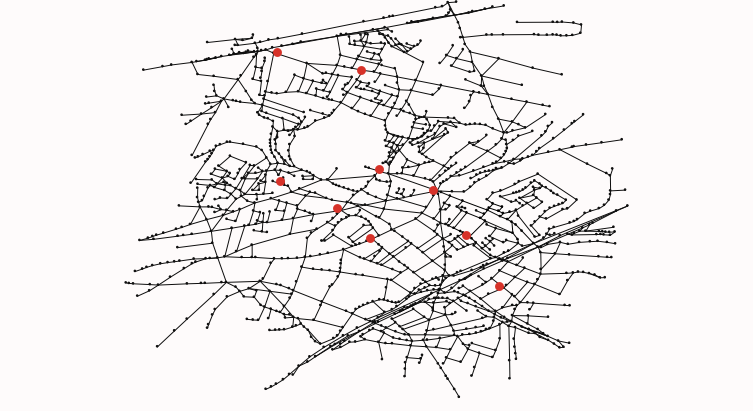
\includegraphics[width=0.32\textwidth]{figures/slimemould_tick1}
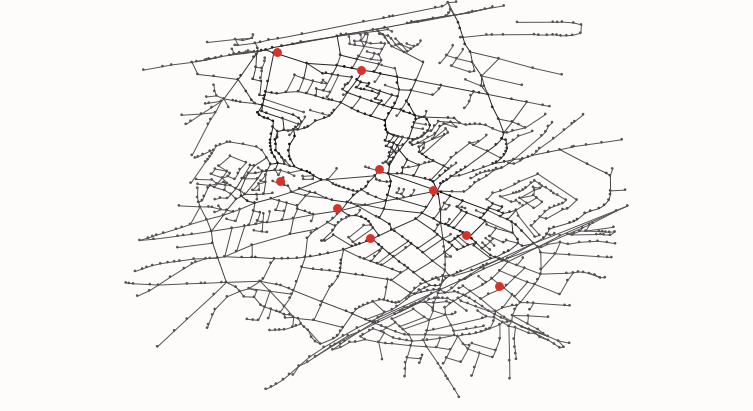
\includegraphics[width=0.32\textwidth]{figures/slimemould_tick10}
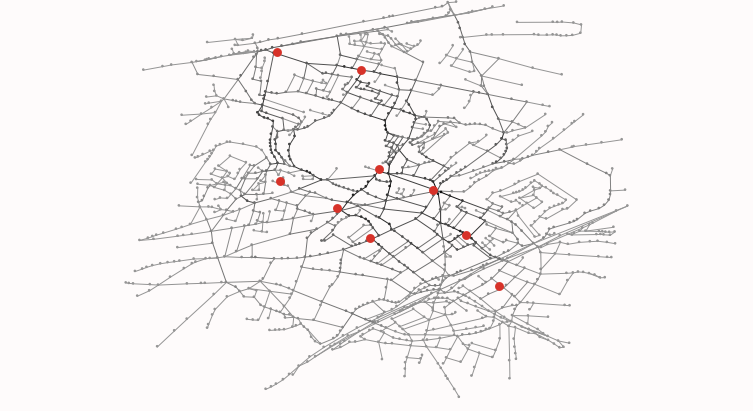
\includegraphics[width=0.32\textwidth]{figures/slimemould_tick20}\\
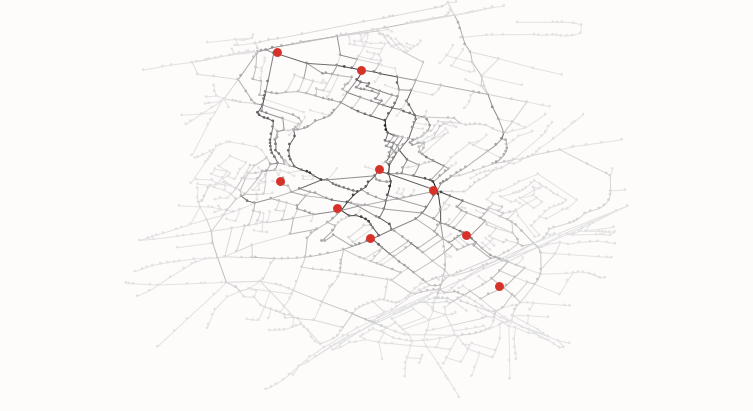
\includegraphics[width=0.32\textwidth]{figures/slimemould_tick50}
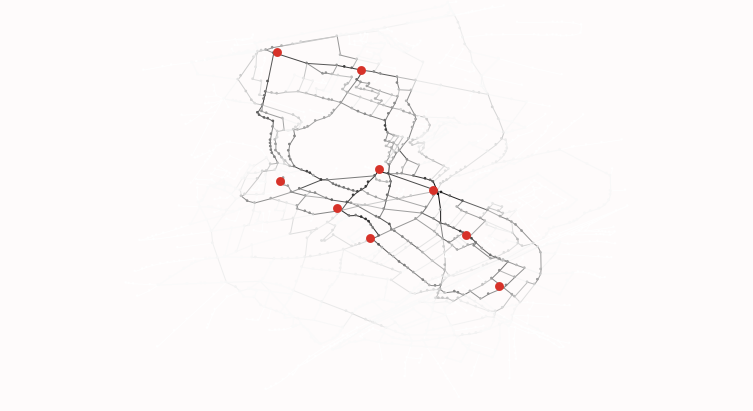
\includegraphics[width=0.32\textwidth]{figures/slimemould_tick101}
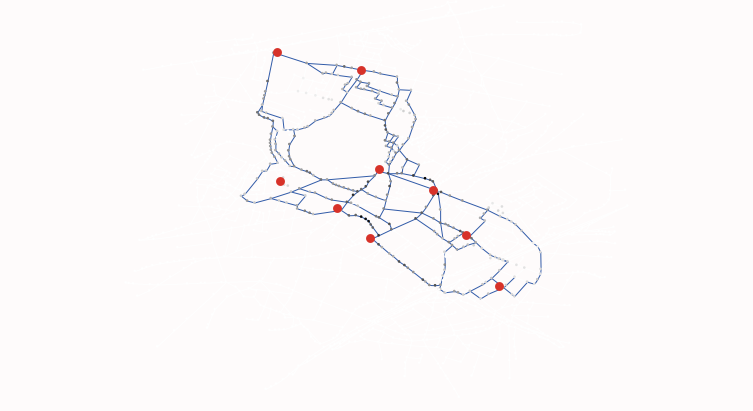
\includegraphics[width=0.32\textwidth]{figures/slimemould_reseauFinal}\\

\medskip

\footnotesize
\textit{Application to the design of optimal bus routes}

}





\sframe{Biological Network generation}{

Adding new links with biological heuristic:

\begin{enumerate}
	\item Create network of potential new links, with existing network and randomly sampled diagonal lattice
	\item Iterate for $k$ increasing ($k\in \{ 1,2,4 \}$ in practice) :
	\begin{itemize}
		\item Using population distribution, iterate $k\cdot n_b$ times the slime mould model to compute new link capacities
		\item Delete links with capacity under $\theta_d$
		\item Keep the largest connected component
	\end{itemize}
	\item Planarize and simplify final network
\end{enumerate}

\medskip

\centering

\frame{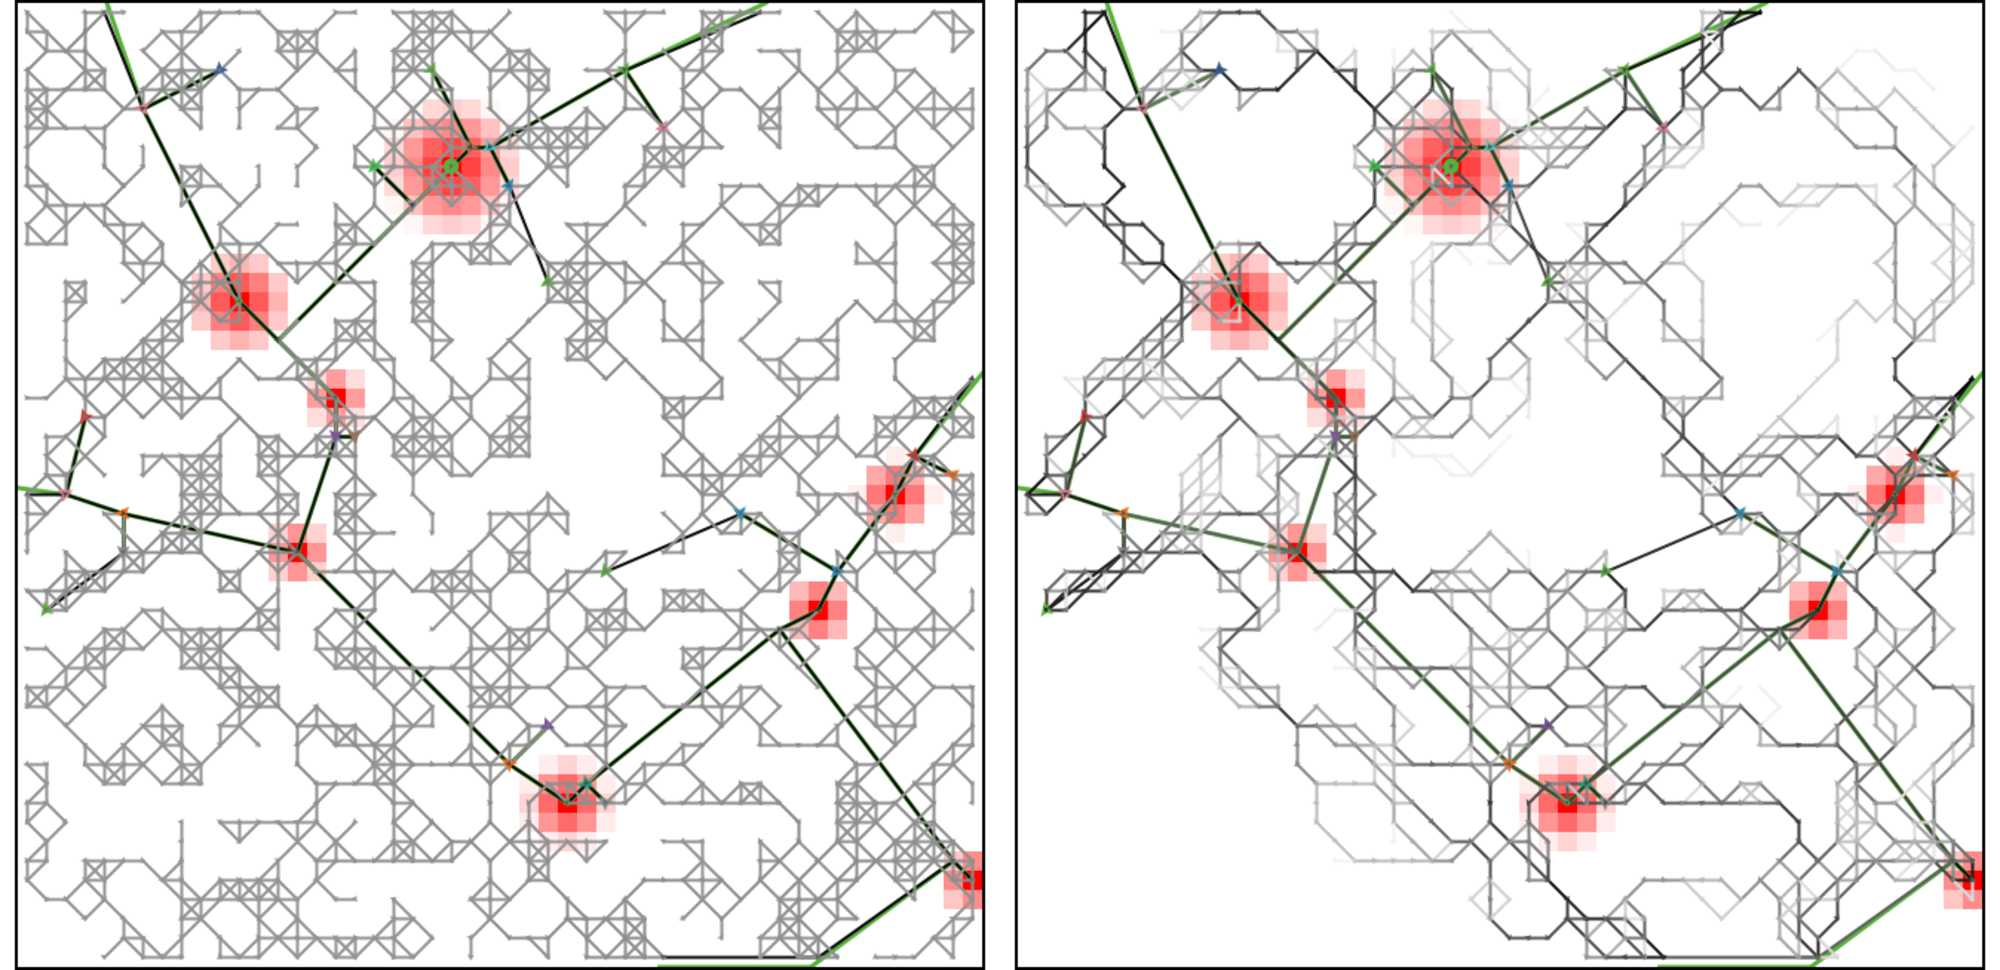
\includegraphics[width=0.6\textwidth]{figures/7-1-1-fig-networkgrowth-bioexample.jpg}}

\footnotesize

\textit{Intermediate stage for biological network generation}

}


\section{Implementation}


\sframe{Model parameters}{

\centering

\vspace{-0.2cm}
\begin{tabular}{|p{1.5cm}|c|c|c|c|c|}
  \hline
Heuristic & Param. & Name & Process & Domain & Default\\
  \hline
\multirow{5}{*}{Base}& $l_m$ & added links & growth & $[0;100]$ & $10$ \\\cline{2-6}
 & $d_G$ & gravity distance & potential & $]0;5000]$ & $500$ \\\cline{2-6}
 & $d_0$ & gravity shape & potential & $]0;10]$ & $2$ \\\cline{2-6}
 & $k_h$ & gravity weight & potential & $[0;1]$ & $0.5$ \\\cline{2-6}
 & $\gamma_G$ & gravity hierarchy & potential & $[0.1;4]$ & $1.5$ \\\hline
\multirow{2}{*}{Random}& $\gamma_R$ & random selection  & hierarchy & $[0.1;4]$ & $1.5$ \\\cline{2-6}
& $\theta_R$ & random threshold & breakdown & $[1;5]$ & $2$ \\\hline
Cost-benefits & $\lambda$ & compromise & compromise & $[0;0.1]$ & $0.05$ \\\hline
\multirow{2}{*}{Biological}& $n_b$ & iterations & convergence & $[40;100]$ & $50$ \\\cline{2-6}
& $\theta_b$ & biological th.& threshold & $[0.1;1.0]$ & $0.5$ \\\hline
\end{tabular}

}



\sframe{Model setup}{

\textbf{Synthetic setup: } rank-sized monocentric cities, simple connection with bord nodes to avoid bord effects 

\textbf{Real setup: } Population density raster at 500m resolution (European Union, from Eurostat)

\bigskip

\centering
\frame{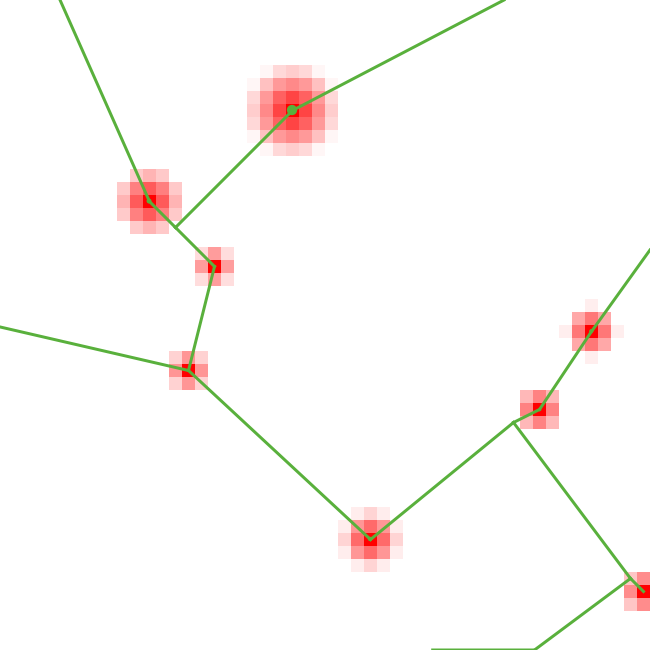
\includegraphics[width=0.35\textwidth]{figures/coevol_example_synthsetup}}\hspace{0.1cm}
\frame{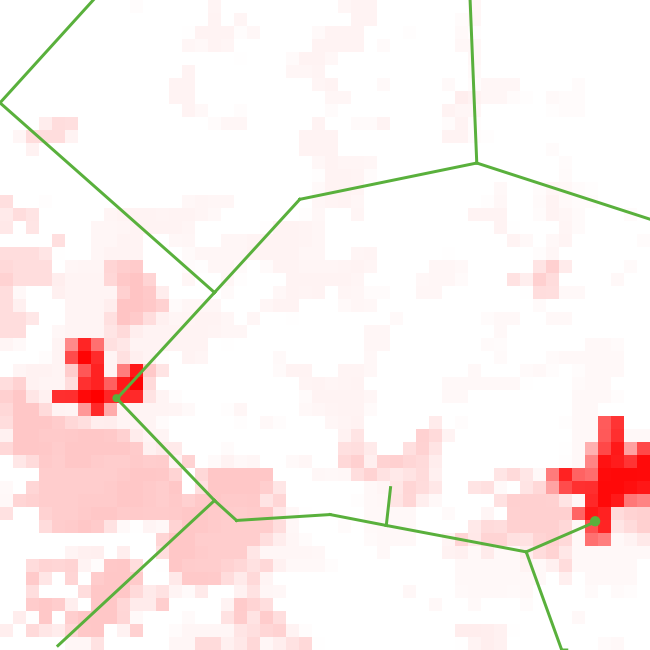
\includegraphics[width=0.35\textwidth]{figures/coevol_example-realsetup}}

\textbf{Stopping conditions: } fixed final time; fixed total population; fixed network size.

}


\sframe{Network Indicators}{

Network Topology measured by:

\begin{itemize}
	\item Betweenness and Closeness centralities: average and hierarchy
	\item Accessibility (weighted closeness)
	\item Efficiency (network pace relative to euclidian distance)
	\item Mean path length, diameter
\end{itemize}

}






\section{Results}

\sframe{Example of generated networks}{

\centering

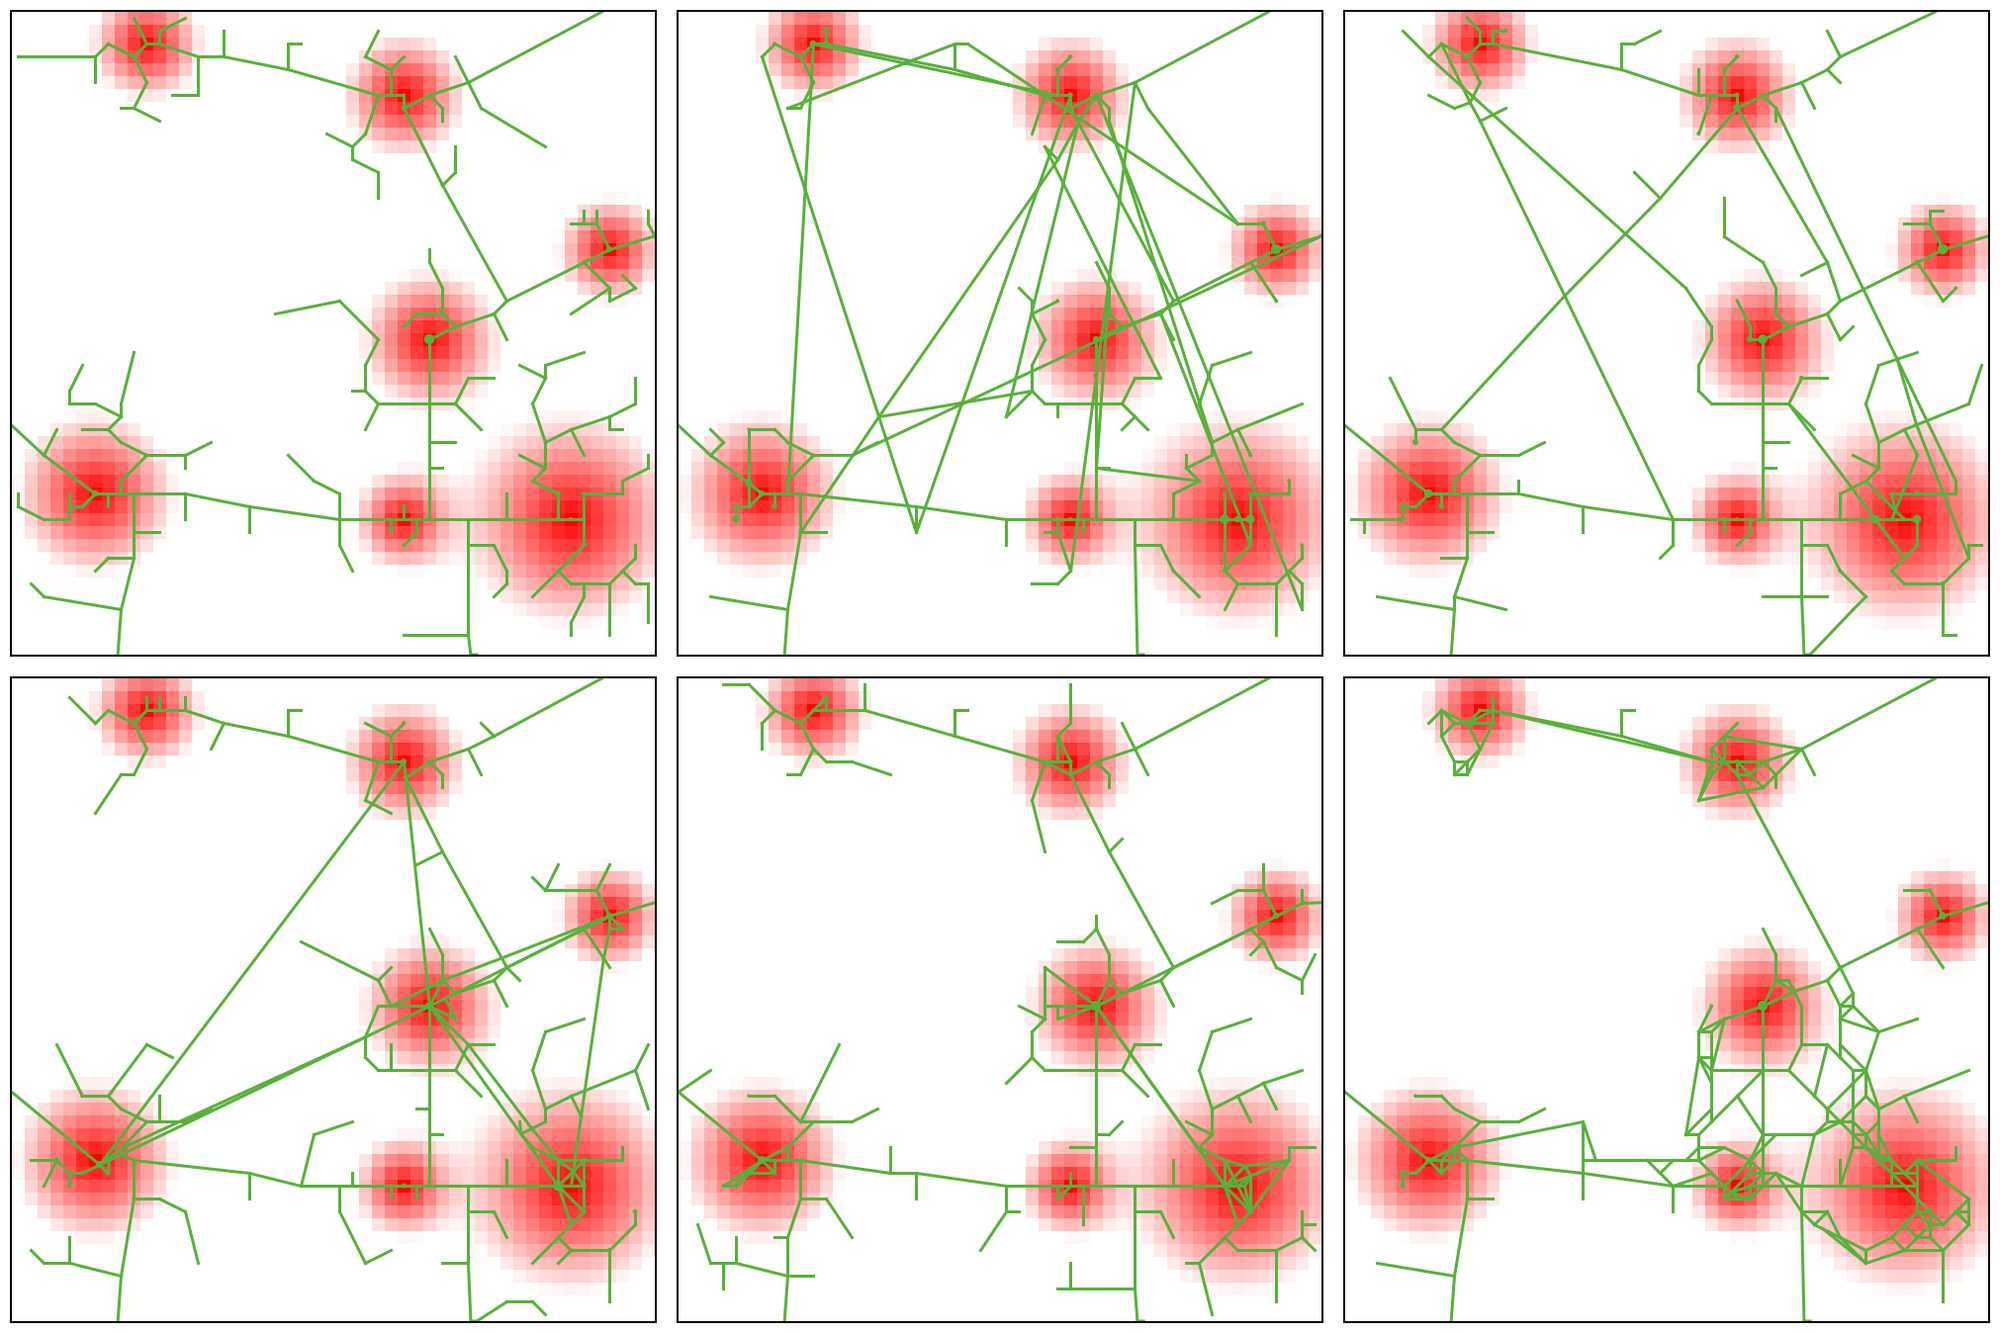
\includegraphics[width=\textwidth]{figures/7-1-2-fig-networkgrowth-examples.jpg}

\footnotesize\textit{In order: connection; random; deterministic breakdown; random breakdown; cost-driven; biological.}

}


\sframe{Pattern Space Exploration algorithm}{

}


\sframe{Indicators feasible space}{

}


\sframe{Hypervolumes}{

}




\sframe{Conclusion}{


\justify

$\rightarrow$ 

\medskip

$\rightarrow$ 

\bigskip
\bigskip



\textbf{Open repositories}

\medskip

\url{https://github.com/JusteRaimbault/NetworkGrowth} 




}






%%%%%%%%%%%%%%%%%%%%%
\begin{frame}[allowframebreaks]
\frametitle{References}
\bibliographystyle{apalike}
\bibliography{biblio}
\end{frame}
%%%%%%%%%%%%%%%%%%%%%%%%%%%%










\end{document}





